\chapter{システムの提案}
\label{chap:proposal}

本章では,音声利用についての背景を踏まえ,新しい録音システム「Gyaon」を提案する.

\newpage

\section{設計指針}

Gyaonでは
\begin{enumerate}
\item 単純な録音操作
\item 音声管理の簡単さ
\item 他システムからの音声の利用のしやすさ
\end{enumerate}
を優先した設計を行うことで録音の不便を解消し,音声の有効活用を促すシステムを目指している.

\section{利用例}
様々な利用シーンに対応するため,PC用Webアプリケーションおよび
Androidスマートフォン用アプリケーション
にてGyaonシステムが利用できる.
それぞれのプラットフォームにおける利用例を述べる.

\subsection{PC版}

\subsubsection{基本操作}
PC版Gyaonはhttps://gyaon.herokuapp.com/にて試験運用しており,Webブラウザで動作する.
図\ref{gyaon}が起動画面である.
録音ボタンを押している間だけ録音され,停止後にプレビュー再生が行われる.
同時に音声データがサーバへアップロードされる.
アップロードが完了したものは音声リストに表示され,マウスカーソルを重ねるだけで再生できる.

\begin{figure}[H]
\centering
\fbox{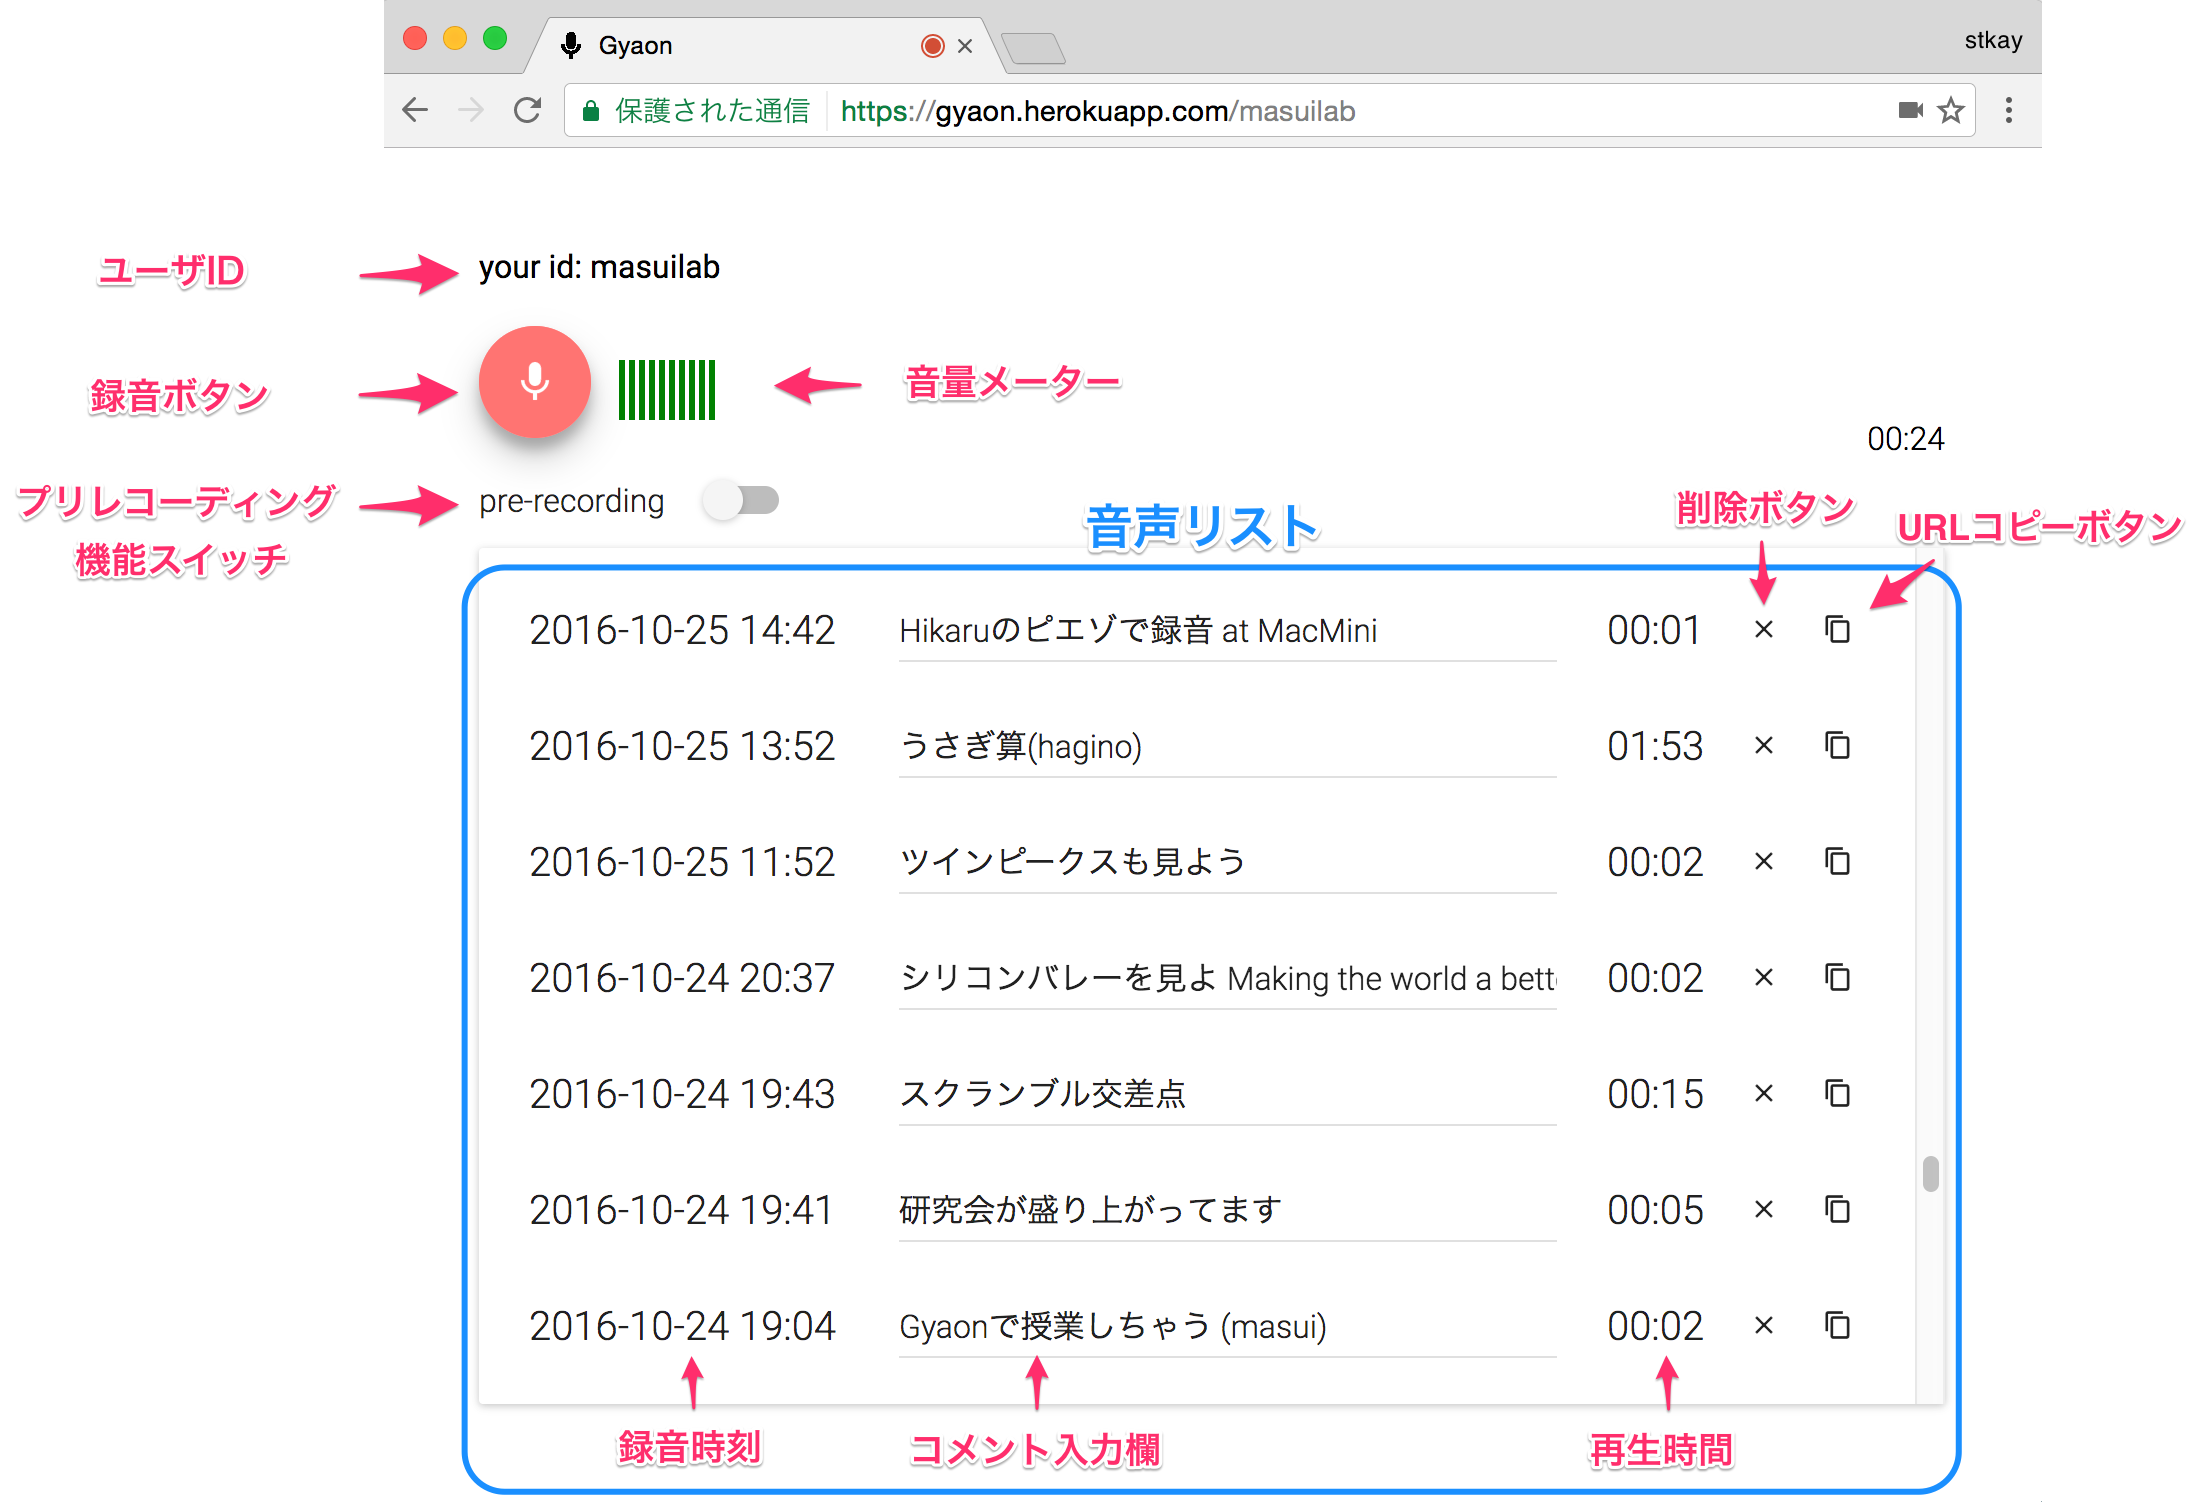
\includegraphics[width=15cm]{images/gyaon.png}}
\caption{PC版Gyaonの起動画面}
\label{gyaon}
\end{figure}

\subsubsection{コメントの追加}
音声リスト内のコメント入力欄をクリックすると,コメント入力モードに移行する.
音声の内容などを自由に記録することができる.

\subsubsection{音声URLの取得}
音声リスト右側のコピーボタンをクリックすることで,
PCのクリップボードに音声データのURLがコピーされる.
そのままアクセスすれば音声をダウンロードでき,ローカル環境のアプリケーションなどで利用できるほか,
URLを経由して他人に音声を渡すことも可能である.
またNota.inc\footnote{\textsf{http://www.notainc.com/ja/}}のWikiシステム
「Scrapbox」\footnote{\textsf{https://scrapbox.io/}}ではオーディオ記法を利用でき,
決められた書式で音声のURLを入力すると,Gyaonの音声リストと同様にマウスカーソルによる再生が可能となる.

\begin{figure}[H]
\centering
\fbox{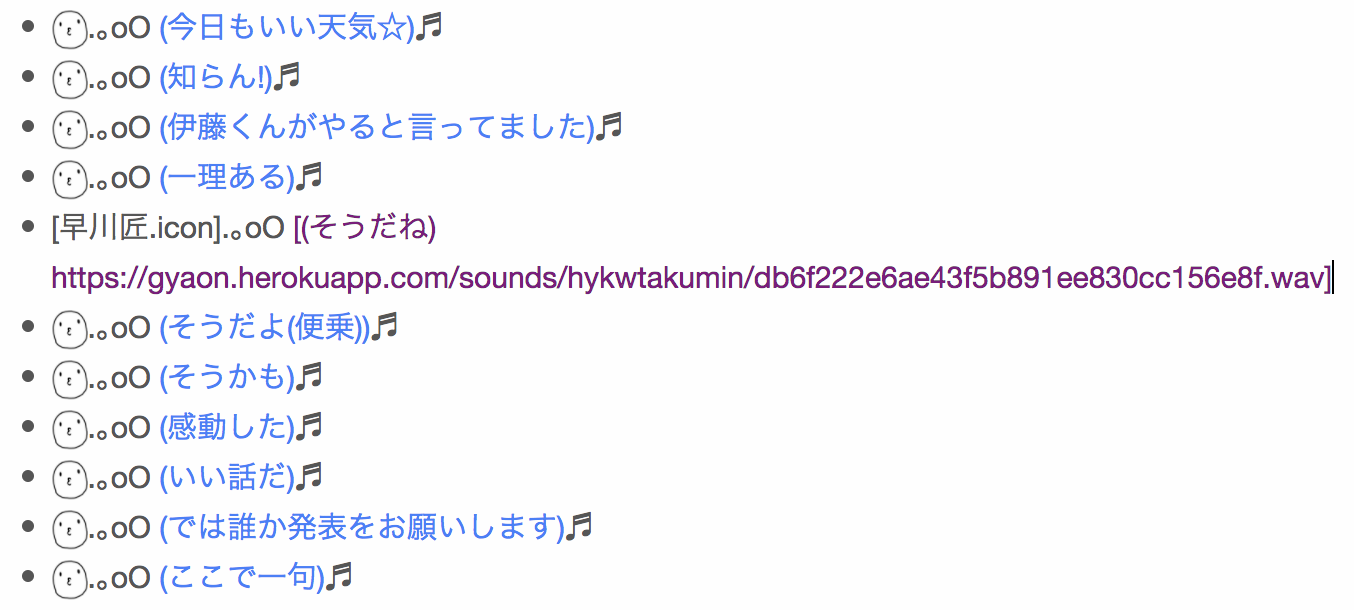
\includegraphics[width=9cm]{images/scrapbox.png}}
\caption{Scrapboxのオーディオ記法}
\label{scrapbox}
\end{figure}

\subsubsection{プリレコーディング機能}
「pre-recording」スイッチをONにするとアプリ起動中は常時録音し,
録音ボタンを押す10秒前から音声を記録できる.
もし突然録りたい音が聞こえてきた場合でも後から録音することが可能である.
%今いいこと言った!を逃さない
%急に面白い音が聞こえてきても逃さない

\subsubsection{地図機能}
音声データに紐付けられた位置情報をもとに,音声を地図上にマッピングして一覧できる
\footnote{\textsf{地図機能はhttps://gyaon.herokuapp.com/map/にて試験運用中}}.
音声の録音場所が分かることから,その場所の雰囲気や,
景色がいい/この店は美味しいといったその場所ならではの有用な情報を記録/共有できる.

\begin{figure}[H]
\centering
\fbox{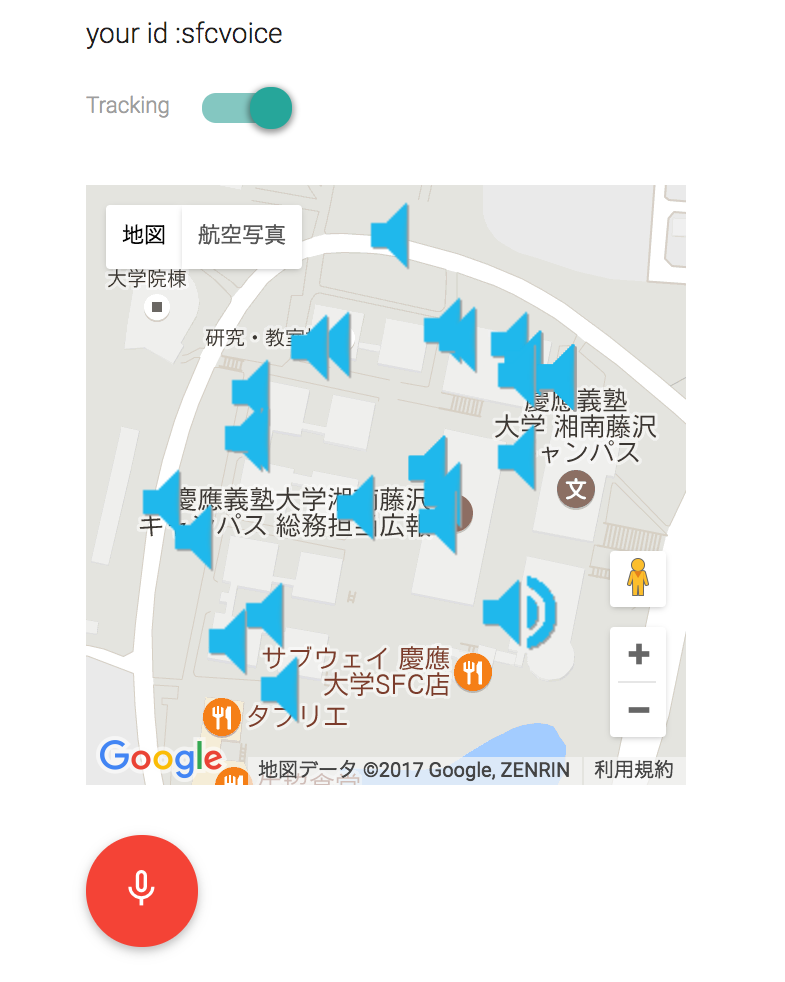
\includegraphics[width=9cm]{images/map.png}}
\caption{地図機能}
\label{map}
\end{figure}

\subsubsection{IDの共有}
GyaonではIDごとに音声を管理しており,ログインは不要で,URL末尾でユーザIDを指定できる.
もしユーザIDを指定せずにGyaonにアクセスした場合,ランダムの文字列がユーザIDとして割り当てられる.
このIDを複数人で共有することでGyaonを共有タスクリストのように利用したり,
ボイスメッセンジャーのような使い方が可能である.

\begin{itembox}[l]
{ユーザIDの指定}
https://gyaon.herokuapp.com/\{ユーザID\}
\end{itembox}

\subsubsection{Gyaonキー}
Gyaonキーアプリケーション\footnote{\textsf{Mac用アプリケーションをhttps://github.com/stkay/GyaonWithKarabinerにて配布中}}
を利用すれば,PCの任意のキーを録音ボタンに設定できる.
これにより,アプリケーションを起動することなく録音可能である.
Webアプリケーションと同様に押している間録音が行われ,終了と同時にアップロードが行われる.
%キーボードじゃなくて,他の汎用なボタンでもいいよね

\begin{figure}[H]
\centering
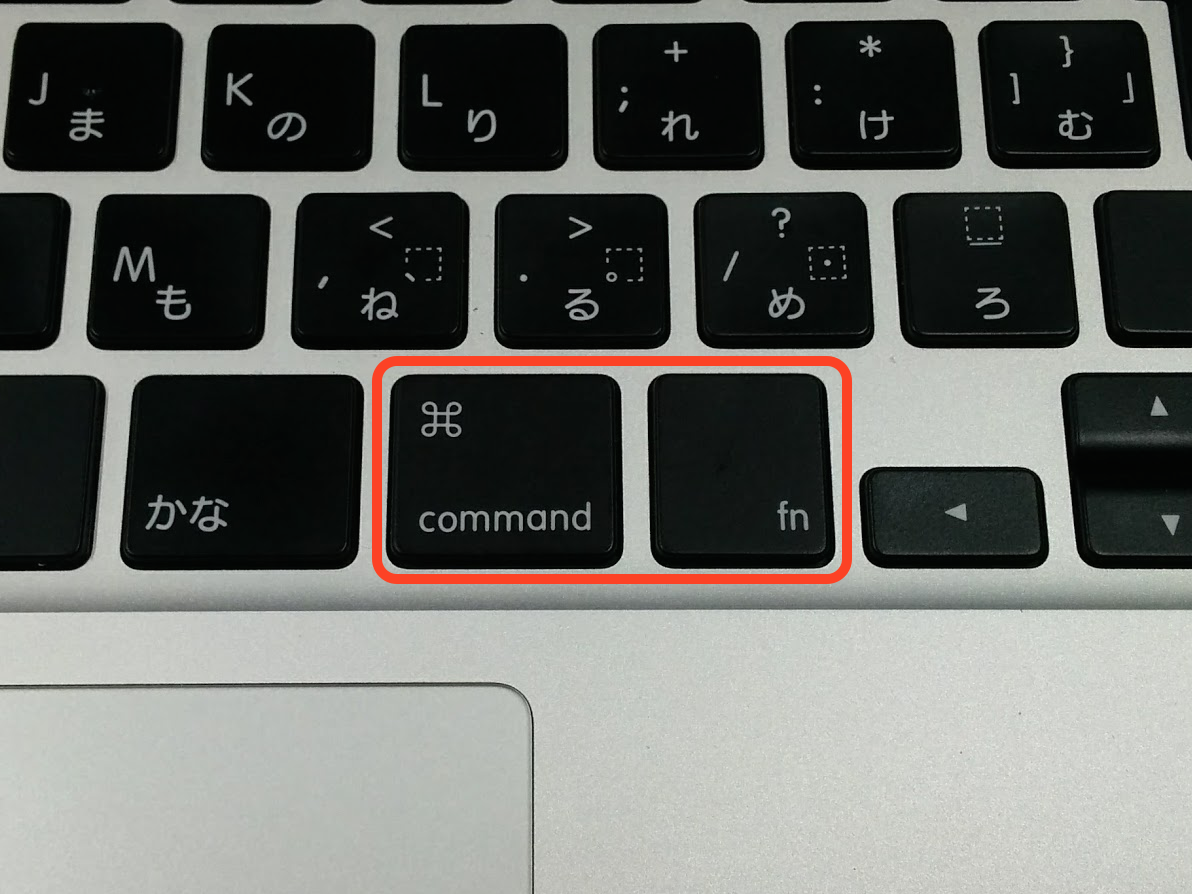
\includegraphics[width=9cm]{images/key.png}
\caption{著者のPCのGyaonキー}
\label{key}
\end{figure}

\subsubsection{Gyaonペダル}
USB接続の汎用なペダル(図\ref{pedal})を接続すれば,楽器演奏中/運転中/料理中といった手を使えないシーンでも
ハンズフリー録音が可能となる.
また,ペダルとマイクを接続したRaspberry Pi等を複数用意し,録音専用コンピュータとしてセットアップすることで,
ユビキタスな録音環境を自宅や研究室等に構築可能である.

%冷蔵庫の前に置いて在庫管理,買い物メモ
%トイレ
%キーボードが使えないけどよくいる場所

\begin{figure}[H]
\centering
\fbox{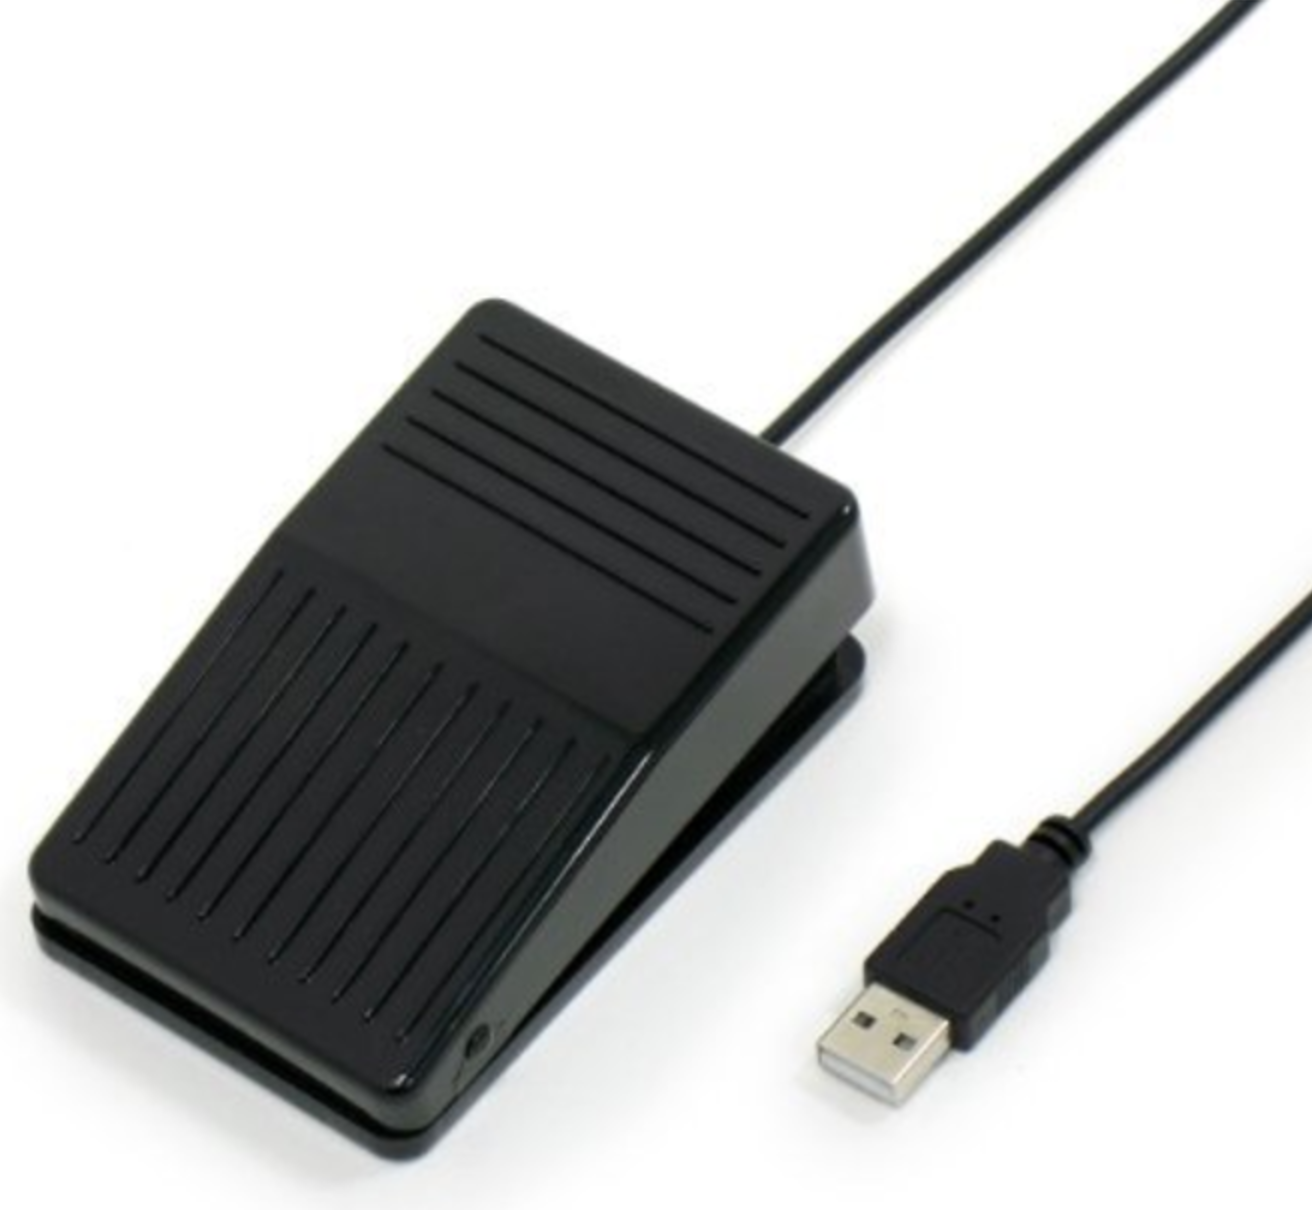
\includegraphics[width=9cm]{images/pedal.png}}
\caption{ペダルの例}
\label{pedal}
\end{figure}

%楽器弾きながらペダル踏んでる画像があるといいかも

\subsection{Android版}

\subsubsection{基本操作}
Android用Gyaonアプリケーションは録音のみ可能で,PC版と同様に押している間録音/自動アップロードが利用できる.(図\ref{app}).
「Your ID」には任意のユーザIDを入力する.
PC版で使用しているユーザIDを入力すれば,スマートフォンでの録音をPCでも聞けるようになる.

\subsubsection{録音ボタンを常駐させる}
図\ref{app}の「STARTSERVICE」ボタンを押すと,録音ボタンをスマートフォン上に常駐させることができる(図\ref{home}).

\subsubsection{利用シーン}
スマートフォンを持ち運べる環境ならいつでもどこでも録音可能である.
外出先で思いついたことを記録したり,
鳥のさえずり/川のせせらぎといった環境音や,アナウンス/街頭演説といった情報を共有する用途にも活用できる.

\begin{figure}[H]
\centering
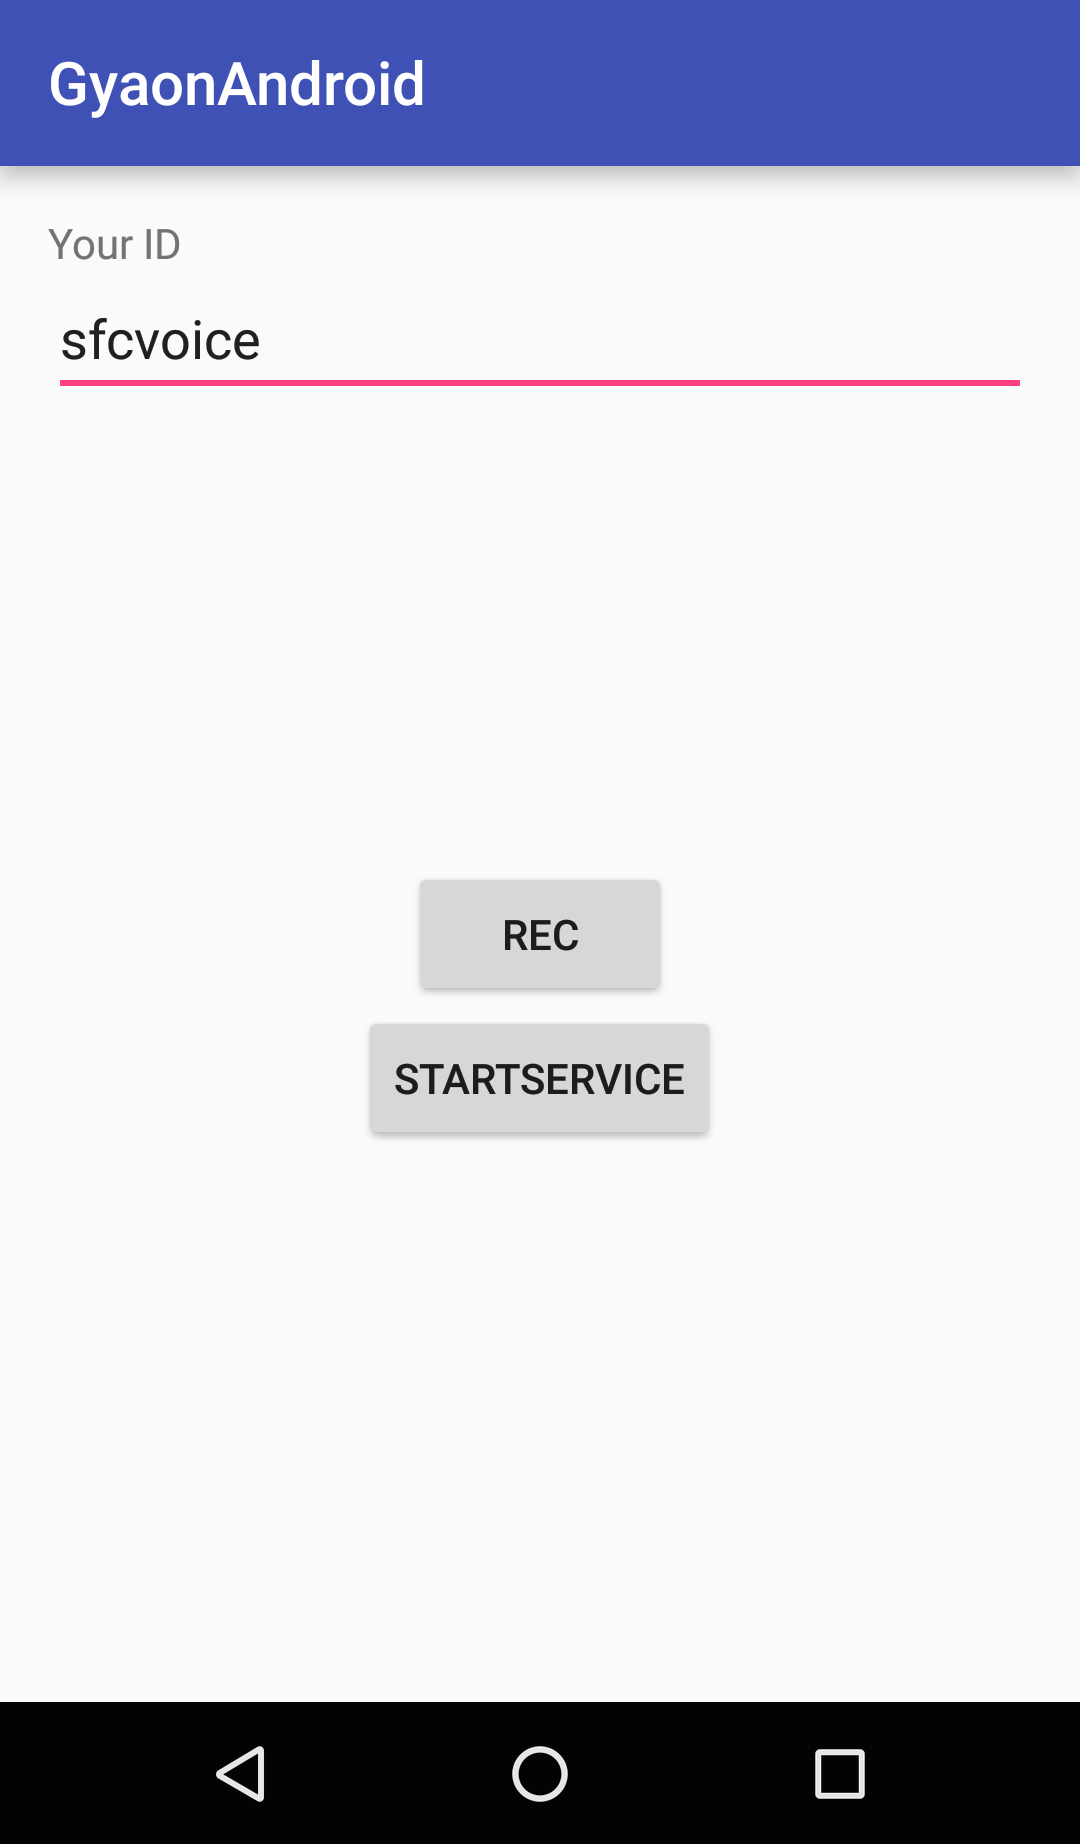
\includegraphics[width=6cm]{images/app.png}
\caption{アプリケーションの起動画面}
\label{app}
\end{figure}

\begin{figure}[H]
\centering
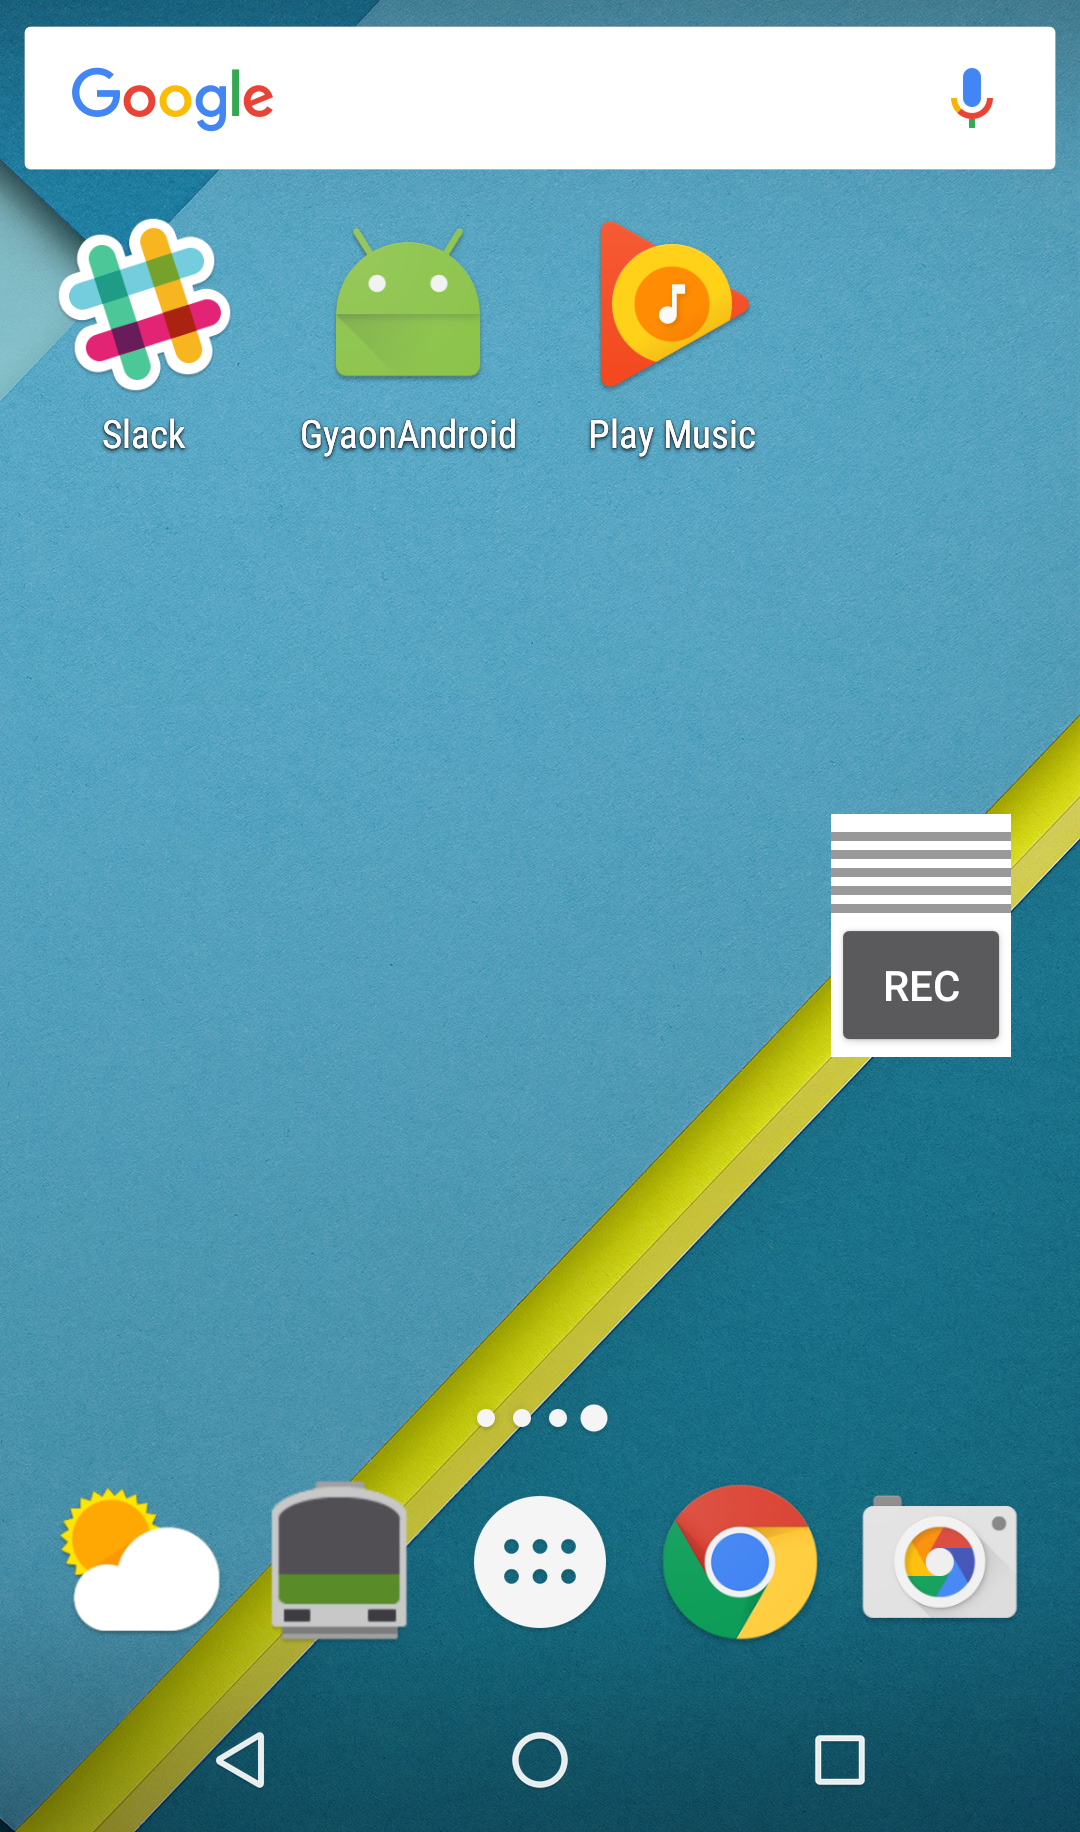
\includegraphics[width=6cm]{images/home.png}
\caption{録音ボタンが配置されたAndroidのホーム画面}
\label{home}
\end{figure}